\documentclass[12pt]{article}
\usepackage[utf8]{inputenc}
\usepackage[T1]{fontenc}
\usepackage{indentfirst}
\usepackage{amsmath}
\usepackage{amssymb}
\usepackage{natbib}
\usepackage{graphicx}
\usepackage{float}
\usepackage[a4paper, margin = 2 cm]{geometry}
\usepackage{fancyhdr}
\usepackage{wrapfig}
\usepackage{hyperref}
\usepackage{mathtools}
\usepackage{tikz}

\title{Computational complexity assignment 2}
\author{Dominik Wawszczak}
\date{2024-10-31}

\begin{document}
	\setlength{\parindent}{0 cm}
	
	Dominik Wawszczak \hfill Computational Complexity
	
	student id number: 440014 \hfill assignment 2
	
	group number: 3
	
	\bigskip
	\hrule
	\bigskip
	
	\textbf{Task 1}
	
	\medskip
	
	To begin, we will show that verifying whether an input contains a tree can
	be checked using \(\mathcal{O}(\log N)\) space, where \(N\) is the size of
	the input. A graph is a tree if and only if it satisfies the following two
	conditions:
	\begin{enumerate}
		\item The number of edges is one less than the number of vertices.
		\item The graph is connected.
	\end{enumerate}
	Checking the first condition is straightforward. We can iterate over the
	edges while maintaining a binary counter and then verify if it equals
	\(n - 1\). This counter will indeed require no more than
	\(\mathcal{O}(\log N)\) space.
	
	\medskip
	
	The second condition is more complex. We can iterate over all pairs \((s, t)
	\in \{1, \ldots, n\}^{2}\) using two binary counters. For each pair, we need
	to determine if a simple path exists from \(s\) to \(t\). This problem
	belongs to the L class, as discussed in the lecture.
	
	\medskip
	
	A \textit{root} of a tree \(T\) with radius at most \(2\) is a vertex \(r
	\in V(T)\) such that every other vertex in \(V(T)\) is within distance \(2\)
	of \(r\).
	
	\medskip
	
	We will use a slightly different definition of an \textit{induced subgraph}
	than the one in the assignment statement. A graph \(G_{1}\) is an induced
	subgraph of \(G_{2}\) if and only if there exists an injection \(f :
	V(G_{1}) \to V(G_{2})\) such that
	\[ \underset{u \in V(G_{1})}{\forall} \ \underset{v \in V(G_{1})}{\forall} \
	(u, v) \in E(G_{1}) \ \iff \ (f(u), f(v)) \in E(G_{2}) \text{,} \]
	which we will refer to as the \textit{map function}.
	
	\medskip
	
	Our approach will follow these steps:
	\begin{enumerate}
		\item Find a root \(r\) of \(T_{1}\).
		      
		      To do this, iterate over all vertices of \(T_{1}\), treating each
		      vertex as a candidate for \(r\). To verify a candidate, check for
		      each \(v \in V(T_{1}) \setminus \{r\}\) whether either \((v, r)
		      \in E(T_{1})\) or there exists a vertex \(u \in V(T_{1}) \setminus
		      \{v, r\}\) with \((v, u) \in E(T_{1})\) and \((u, r) \in
		      E(T_{1})\).
		      
		      This requires three binary counters (for \(r\), \(v\), and \(u\)).
		      If no root is found, we can reject the input.
		
		\item For each \(s \in V(T_{2})\), check if there exists a valid map
		      function \(f\) such that \(f(r) = s\).
		      
		      The remaining part of the solution will focus on this check.
	\end{enumerate}
	
	\underline{Lemma 1} Let \(T_{1}\) be a tree of radius \(2\) with root \(r\),
	and let \(T_{2}\) be any tree. Let \(v_{1}, \ldots, v_{k}\) denote the
	children of \(r\), ordered so that
	\[ \underset{i \in \{2, \ldots, k\}}{\forall} \ (\deg(v_{i - 1}), v_{i - 1})
	\ \geqslant \ (\deg(v_{i}), v_{i}) \text{,} \]
	where
	\[ (a_{1}, b_{1}) \ \geqslant \ (a_{2}, b_{2}) \quad \iff \quad a_{1} >
	a_{2} \ \vee \ (a_{1} = a_{2} \ \wedge \ b_{1} \geqslant b_{2}) \text{.} \]
	Let \(s\) be any vertex of \(T_{2}\), and denote \(u_{1}, \ldots, u_{l}\)
	as the children of \(s\) when \(T_{2}\) is rooted at \(s\), ordered
	similarly. Then a map function \(f\) with the property that \(f(r) = s\)
	exists if and only if
	\begin{equation} \label{eq:eq1}
		k \ \leqslant \ l \quad \wedge \quad \underset{i \in \{1, \ldots, k\}}
		{\forall} \ \deg(v_{i}) \ \leqslant \ \deg(u_{i}) \text{.}
	\end{equation}
	
	\underline{Proof of Lemma 1} If condition (\ref{eq:eq1}) holds, we can define
	\(f(r) = s\) and set \(f(v_{i}) = u_{i}\) for each \(i \in \{1, \ldots,
	k\}\), ensuring there are enough vertices in \(T_{2}\) to accommodate each
	grandson of \(r\).
	
	\medskip
	
	To derive a contradiction, assume there is a map function \(f\), but
	condition (\ref{eq:eq1}) does not hold. Since \(k \leqslant l\) must be
	true, there exists an \(i \in \{1, \ldots, k\}\) such that \(\deg(v_{i}) >
	\deg(u_{i})\). Take the smallest such \(i\). There is a unique \(j\)
	such that \(f(v_{i}) = u_{j}\), which must be less than \(i\), or there
	would not be enough vertices to match the children of \(v_{i}\); thus \(i >
	1\). For each \(i' < i\), let \(j'\) be the index with \(f(v_{i'}) =
	u_{j'}\); similarly, \(j'\) must be less than \(i\) because \(\deg(v_{i'})
	\geqslant \deg(v_{i})\). This creates a contradiction by the Pigeonhole
	principle, as \(f\) was assumed to be injective, completing the proof.
	
	\medskip
	
	Returning to the second step, once we have the root \(r\), finding the
	number \(k\) of its children requires only one binary counter. For a given
	\(s \in V(T_{2})\), we can similarly find the number of its children \(l\).
	By Lemma 1, if \(k > l\), we can discard \(s\) as a candidate. Otherwise, we
	need to verify for each \(i \in \{1, \ldots, k\}\) whether \(\deg(v_{i})
	\leqslant \deg(u_{i})\). To calculate the degree of a vertex, we can iterate
	over edges while using a single binary counter. However, finding \(v_{i}\)
	and \(u_{i}\) in logarithmic space is more challenging.
	
	\medskip
	
	We can determine \((\deg(v_{1}), v_{1})\) by iterating over the sons of
	\(r\), comparing each \((\deg(v_{\text{cur}}), v_{\text{cur}})\) with the
	best pair found so far, and updating as needed. We can calculate
	\((\deg(u_{1}), u_{1})\) in a similar way. After this, we compare
	\(\deg(v_{1}) \leqslant \deg(u_{1})\) and reject if the condition does not
	hold; otherwise, we move on to the next pair. Once \((\deg(v_{i}), v_{i})\)
	is calculated, obtaining \((\deg(v_{i + 1}), v_{i + 1})\) is straightforward
	-- simply ignore any \((\deg(v_{\text{cur}}), v_{\text{cur}})\) strictly
	greater than \((\deg(v_{i}), v_{i})\). The same process applies to
	\((\deg(u_{i + 1}), u_{i + 1})\).
	
	\medskip
	
	The entire algorithm requires only a constant number of binary counters,
	concluding the solution.
	
	\bigskip
	
	\textbf{Task 2}
	
	\medskip
	
	To start, we will prove that the language belongs to the NP class. For any
	induced subgraph \(H\) of \(G\), we need to perform the following steps:
	\begin{enumerate}
		\item Verify that \(H\) is a tree.
		\item Identify the root of \(H\), confirming that \(H\) is a tree of
		      radius \(2\).
		\item Compare the multisets of degrees of the children of the roots in
		      both \(T\) and \(H\).
	\end{enumerate}
	Each of these steps can be completed in polynomial time.
	
	\medskip
	
	Now, we proceed to show that the problem is NP-hard. To do so, we will
	construct a Karp reduction from the \(3\)-coloring problem to the problem
	specified in the assignment.
	
	\medskip
	
	Let \(G^{\ast}\) be an arbitrary graph. Our goal is to construct a tree
	\(T\) of radius \(2\) and a graph \(G\) such that
	\begin{equation} \label{eq:eq2}
		G^{\ast} \ \text{is 3-colorable} \quad \iff \quad T \ \text{is
		isomorphic to an induced subgraph of} \ G \text{.}
	\end{equation}
	
	\medskip
	
	Let \(n = |V(G^{\ast})|\) and \(m = |E(G^{\ast})|\). The tree \(T\) will
	consist of a root \(r\) and \(n + 3\) children: a vertex \(v'\) for each \(v
	\in V(G^{\ast})\) and three auxiliary vertices: \(a_{1}\), \(a_{2}\), and
	\(a_{3}\).
	
	\newpage
	
	The graph \(G\) will include a special vertex \(s\). For each \(v
	\in V(G^{\ast})\), the following structure will be added to \(G\):
	\begin{center}
		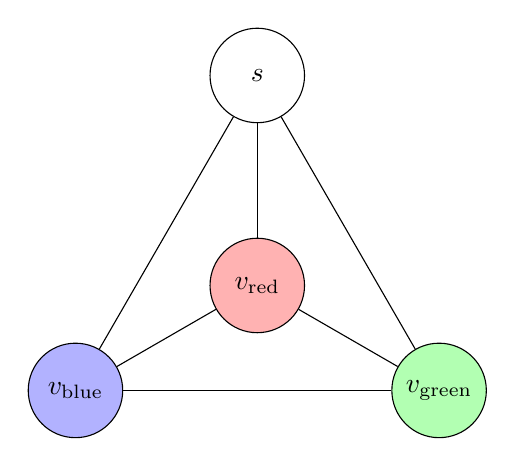
\begin{tikzpicture}
			\tikzset{vertex/.style = {draw, circle, inner sep=0pt,
			minimum size=1.2cm}}
			
			\node[vertex, fill=white] (s) at (0, 0) {\(s\)};
			\node[vertex, fill=blue!30] (v_blue) at (-2.309, -4)
			{\(v_{\text{blue}}\)};
			\node[vertex, fill=green!30] (v_green) at (2.309, -4)
			{\(v_{\text{green}}\)};
			\node[vertex, fill=red!30] (v_red) at (0, -2.667)
			{\(v_{\text{red}}\)};
			
			\draw (s) -- (v_blue);
			\draw (s) -- (v_green);
			\draw (s) -- (v_red);
			\draw (v_blue) -- (v_green);
			\draw (v_blue) -- (v_red);
			\draw (v_green) -- (v_red);
		\end{tikzpicture}
	\end{center}
	Additionally, for each edge \((u, v) \in E(G^{\ast})\), we will add the
	following three edges to \(G\):
	\begin{center}
		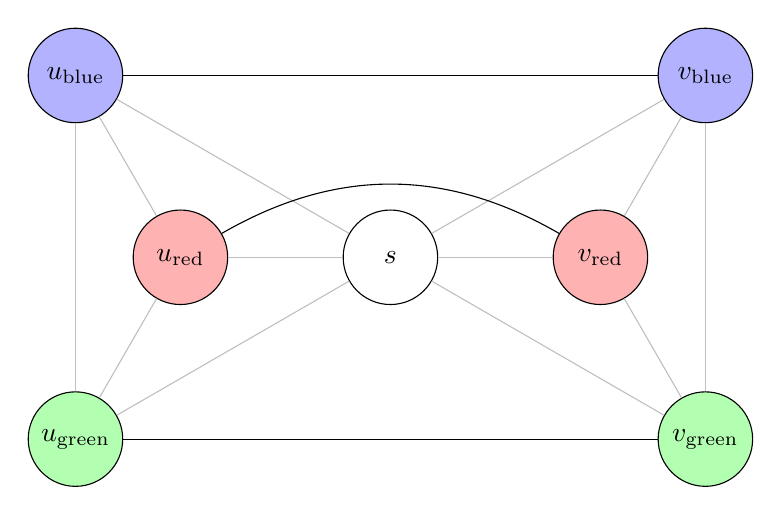
\begin{tikzpicture}
			\tikzset{vertex/.style = {draw, circle, inner sep=0pt,
			minimum size=1.2cm}}
			
			\node[vertex, fill=white] (s) at (0, 0) {\(s\)};
			\node[vertex, fill=blue!30] (u_blue) at (-4, 2.309)
			{\(u_{\text{blue}}\)};
			\node[vertex, fill=green!30] (u_green) at (-4, -2.309)
			{\(u_{\text{green}}\)};
			\node[vertex, fill=red!30] (u_red) at (-2.667, 0)
			{\(u_{\text{red}}\)};
			
			\draw[lightgray] (s) -- (u_blue);
			\draw[lightgray] (s) -- (u_green);
			\draw[lightgray] (s) -- (u_red);
			\draw[lightgray] (u_blue) -- (u_green);
			\draw[lightgray] (u_blue) -- (u_red);
			\draw[lightgray] (u_green) -- (u_red);
			
			\node[vertex, fill=blue!30] (v_blue) at (4, 2.309)
			{\(v_{\text{blue}}\)};
			\node[vertex, fill=green!30] (v_green) at (4, -2.309)
			{\(v_{\text{green}}\)};
			\node[vertex, fill=red!30] (v_red) at (2.667, 0)
			{\(v_{\text{red}}\)};
			
			\draw[lightgray] (s) -- (v_blue);
			\draw[lightgray] (s) -- (v_green);
			\draw[lightgray] (s) -- (v_red);
			\draw[lightgray] (v_blue) -- (v_green);
			\draw[lightgray] (v_blue) -- (v_red);
			\draw[lightgray] (v_green) -- (v_red);
			
			\draw (u_blue) to (v_blue);
			\draw (u_green) to (v_green);
			\draw[bend left=30] (u_red) to (v_red);
		\end{tikzpicture}
	\end{center}
	Finally, \(s\) will have three auxiliary neighbors: \(b_{1}\), \(b_{2}\) and
	\(b_{3}\).
	
	\medskip
	
	It should be noted that the size of the new instance is polynomial in terms
	of the size of \(G^{\ast}\), as \(T\) has \(n + 4\) vertices and \(n + 3\)
	edges, while \(G\) has \(3n + 4\) vertices and \(6n + 3m + 3\) edges.
	Therefore, the only remaining step is to prove the equivalence
	(\ref{eq:eq2}).
	
	\medskip
	
	Assume that \(G^{\ast}\) is 3-colorable. For each \(v \in V(G^{\ast})\), let
	\(\text{color}_{v} \in \{\text{blue}, \text{green}, \text{red}\}\) be the
	color assigned to \(v\). We can then define a map function \(f\) as follows:
	\begin{alignat*}{2}
		f(r) \ &= \ s \text{;} & \quad & \\
		f(v') \ &= \ v_{\text{color}_v} \text{,} & \quad & \text{for any} \ v
		\in V(G^{\ast}) \text{;} \\
		f(a_{i}) \ &= \ b_{i} \text{,} & \quad & \text{for} \ i \in \{1, 2, 3\}
		\text{.}
	\end{alignat*}
	For every child \(t\) of \(r\), we have \((f(r), f(t)) \in E(G)\), so we
	only need to show that for any two children \(t_{1}\) and \(t_{2}\) of
	\(r\), \((f(t_{1}), f(t_{2})) \notin E(G)\). If either \(t_{1}\) or
	\(t_{2}\) is one of the three auxiliary children, this is straightforward.
	Otherwise, assume \(t_{1} = u'\) and \(t_{2} = v'\) for some \(u, v \in
	V(G^{\ast})\). If \((u, v) \notin E(G^{\ast})\), then \(f(t_{1}) =
	u_{\text{color}_{u}}\) and \(f(t_{2}) = v_{\text{color}_{v}}\) are not
	connected. On the other hand, if \((u, v) \in E(G^{\ast})\), then
	\(\text{color}_{u} \neq \text{color}_{v}\), meaning they are also not
	connected.
	
	\medskip
	
	Conversely, assume there exists a map function \(f\). Then we must have
	\(f(r) = s\), as \(\deg(r) = n + 3\) and \(s\) is the only vertex in \(G\)
	with degree at least \(n + 3\). We can verify this since
	\[ \deg(v_{\text{color}}) \ = \ 3 + \deg(v) \ \leqslant \ n + 2 \text{,}
	\quad \text{for any} \ v \in V(G^{\ast}) \ \text{and} \ \text{color} \in
	\{\text{blue}, \text{green}, \text{red}\} \text{,} \]
	and \(\deg(b_{1}) = \deg(b_{2}) = \deg(b_{3}) = 1\).
	
	\medskip
	
	Suppose there exists a vertex \(v \in V(G^{\ast})\) and two distinct colors
	\(\text{color}_{1}, \text{color}_{2} \in \{\text{blue}, \text{green},
	\allowbreak \text{red}\}\), such that both \(v_{\text{color}_{1}}\) and
	\(v_{\text{color}_{2}}\) belong to the image of \(f\). Then the induced
	subgraph would contain a triangle \((s, v_{\text{color}_{1}},
	v_{\text{color}_{2}})\), creating a contradiction. Therefore, at most one of
	\(v_{\text{blue}}\), \(v_{\text{green}}\), or \(v_{\text{red}}\) can belong
	to the image of \(f\).
	
	\medskip
	
	If none of \(v_{\text{blue}}\), \(v_{\text{green}}\), or \(v_{\text{red}}\)
	belongs to the image of \(f\), then the size of the image of \(f\) is at
	most \(n + 3\): consisting of \(s\), \(b_{1}\), \(b_{2}\), \(b_{3}\), and
	one vertex for each of the remaining \(n - 1\) vertices. However, the size
	of the domain of is \(n + 4\), and because \(f\) is an injection, it follows
	that exactly one of \(v_{\text{blue}}\), \(v_{\text{green}}\), or
	\(v_{\text{red}}\) must appear in the image of \(f\) for each \(v \in
	V(G^{\ast})\).
	
	\medskip
	
	For any \(v \in V(G^{\ast})\), let \(\text{color}_{v}\) be the unique
	color in \(\{\text{blue}, \text{green}, \text{red}\}\) such that
	\(v_{\text{color}_v} \in f^{-1}(V(T))\). If, for some \((u, v) \in
	E(G^{\ast})\), \(\text{color}_{u} = \text{color}_{v}\), then the induced
	subgraph would contain a triangle \((s, u_{\text{color}_{u}},
	v_{\text{color}_{v}})\), which again results in a contradiction. Thus, we
	have a valid \(3\)-coloring, completing the proof.
\end{document}
